Questa è l'introduzione.

% https://www.sciencedirect.com/topics/computer-science/security-architecture
\section{Pericoli di esporre un server su internet}

L'architettura di sicurezza del Modello OSI considera 5 classi principali di servizi di sicurezza. Tra queste si hanno: autenticazione, controllo degli accessi, confidenzialità, integrità e non ripudio.
In particolare, questi servizi sono definiti come segue:
\begin{itemize}
    \item autenticazione - il servizio di autenticazione verifica l'identita di un utente o di un sistema
    \item controllo degli accessi - il servizio protegge le risorse di sistema da utenti non autorizzati
    \item confidenzialità - il servizio protegge i dati da rivelazioni non autorizzate
    \item integrità - il servizio protegge i dati da modifiche, aggiunte o rimozioni non autorizzate
    \item non ripudio a.k.a non-repudiation - il servizio assicura che il mittente dell'informazione abbia una notifica di consegna e il destinatario riceva una prova di identità del mittente, in modo tale che nessuno dei due possa successivamente negare di aver processato tali dati
\end{itemize}


\section{Concetti di base}
\subsubsection{Tipologie di reti}
Parlando di una rete di calcolatori, si intende una rete a cui sono connessi due o più computer tramite cui è possibile condividere dati, dispositivi, connessione ad internet, e via dicendo.

Esistono varie tipologie di reti di calcolatori, distinte in base al loro target, che consiste nell'estensione della rete. In base a questo parametro, è possibile distinguere le reti in Local Area Network, Metropolitan Area Network e Wide Area Network. Tutte e tre le tipologie sono relative a una rete fisica.

Un altro tipo di reti è composto dalle reti private virtuali, o Virtual Private Networks, che consiste in una rete di calcolatori le cui connessioni tra i nodi utilizzano reti pubbliche (WAN) come fondamenta su cui realizzare una rete virtuale. Questo tipo di reti permette di realizzare collegamenti privati tra location geograficamente anche molto distanti senza la necessità di posare cavi fisici, ma avvalendosi dell'infrastruttura esistente, garantendo comunque integrità e cifratura dei dati, controllo degli accessi e confidenzialità.

\subsubsection{Il modello OSI}
\begin{figure}[ht]
    \centering
    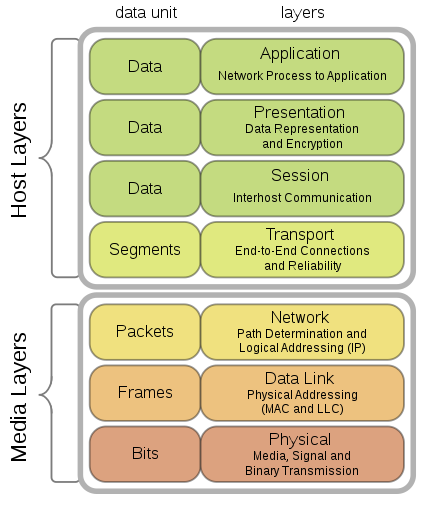
\includegraphics[width=10cm]{figure/osi.png}
    \caption{Modello OSI a strati}
\end{figure}

La pila ISO OSI è uno strumento estremamente efficace nel modellare il funzionamento di una rete di calcolatori.
Si basa su 7 livelli, ognuno dei quali svolge il proprio lavoro utilizzando un'interfaccia standard offerta dal livello inferiore e offrendo a sua volta un'interfaccia al livello superiore.
Tutti e 7 i livelli collaborano per rendere possibile il funzionamento della rete.

I compiti dei sette livelli sono, in breve, i seguenti:
\begin{enumerate}
    \item Livello fisico: è composto dall'infrastruttura fisica - cavi in rame, fibra ottica, ponti radio - e dai componenti hardware che codificano e decodificano i bit
    \item Livello data-link: si occupa di effettuare controlli sul livello fisico, specialmente sull'integrità dei dati
    \item Livello di rete: è il regno del protocollo IP, pilastro delle reti di calcolatori, che si occupa dello smistamento dei pacchetti e di portarli a destinazione
    \item Livello di trasporto: astrae il funzionamento del protocollo IP, offrendo alle applicazioni vari protocolli che si occupano della comunicazione tra due host, indipendentemente da come sono collegati o da quanto sono distanti; può garantire il recapito corretto delle informazioni
    \item Livello di sessione, livello di presentazione, livello di applicazione: sono gli strati più prossimi all'utente finale, e si occupano di gestire la comunicazione dei processi utilizzati dall'utente con il livello di trasporto
\end{enumerate}


\section{Necessità di un'infrastruttura di rete sicura}

Ancora del testo. Come si afferma i
\section{Organizzazione dei capitoli}

Nel capitolo 1, vengono discussi i requisiti del sistema che andranno rispettati nello svolgimento della tesi.
Nel capitolo 2, si discute lo stato dell'arte, illustrando dal punto di vista teorico i protocolli e i software che si andranno ad utilizzare.
Nel capitolo 3, viene illustrata la realizzazione dell'ambiente di test, compresa l'installazione e la configurazione dei servizi scelti.
Nel capitolo 4, si analizzano le misure ottenute durante i test.
Nel capitolo 5, si presentano i principali problemi di sicurezza a cui si potrebbe andare incontro.

